\subsection{Emulation}
In this section, we validate the performance of missing data imputation with the proposed failure localization prediction 
model in an emulated network as shown in Fig.~\ref{fig:topology}. This topology mimics the Internet 2, the US Research 
and Education backbone network that has been used by many large-scale distributed middleware and applications.
It is created in a high-fidelity emulation environment we built in the NSF ExoGENI cloud testbed~\cite{iris:ictc21} 
that can automatically create a virtual network system with virtual machines (VMs) running full software stack, 
bootstrap the network routing, initiate data transfers, and inject arbitrary integrity errors into the virtual router interfaces 
and end hosts to generate labeled training data and test data.

The network consists of 15 end hosts that can originate and receive data transfers and 87 network interfaces that an simulated 
distributed application may transfer data over. The application can check the data integrity of every data transfer at the receiving end hosts.
During the emulation, errors with a given probability will be injected into the every end host and network interfaces in sequence and one hundred 
data transfers are activated between all pairs of the end hosts in each round and the data transfer failure rates are computed. 
Therefore the training data set has 210 features, each of which represents a path between a pair of end hosts. We alter the error probability to generate 
multiple samples that are used to train the regression model.

\begin{figure}[!ht]
\begin{center}
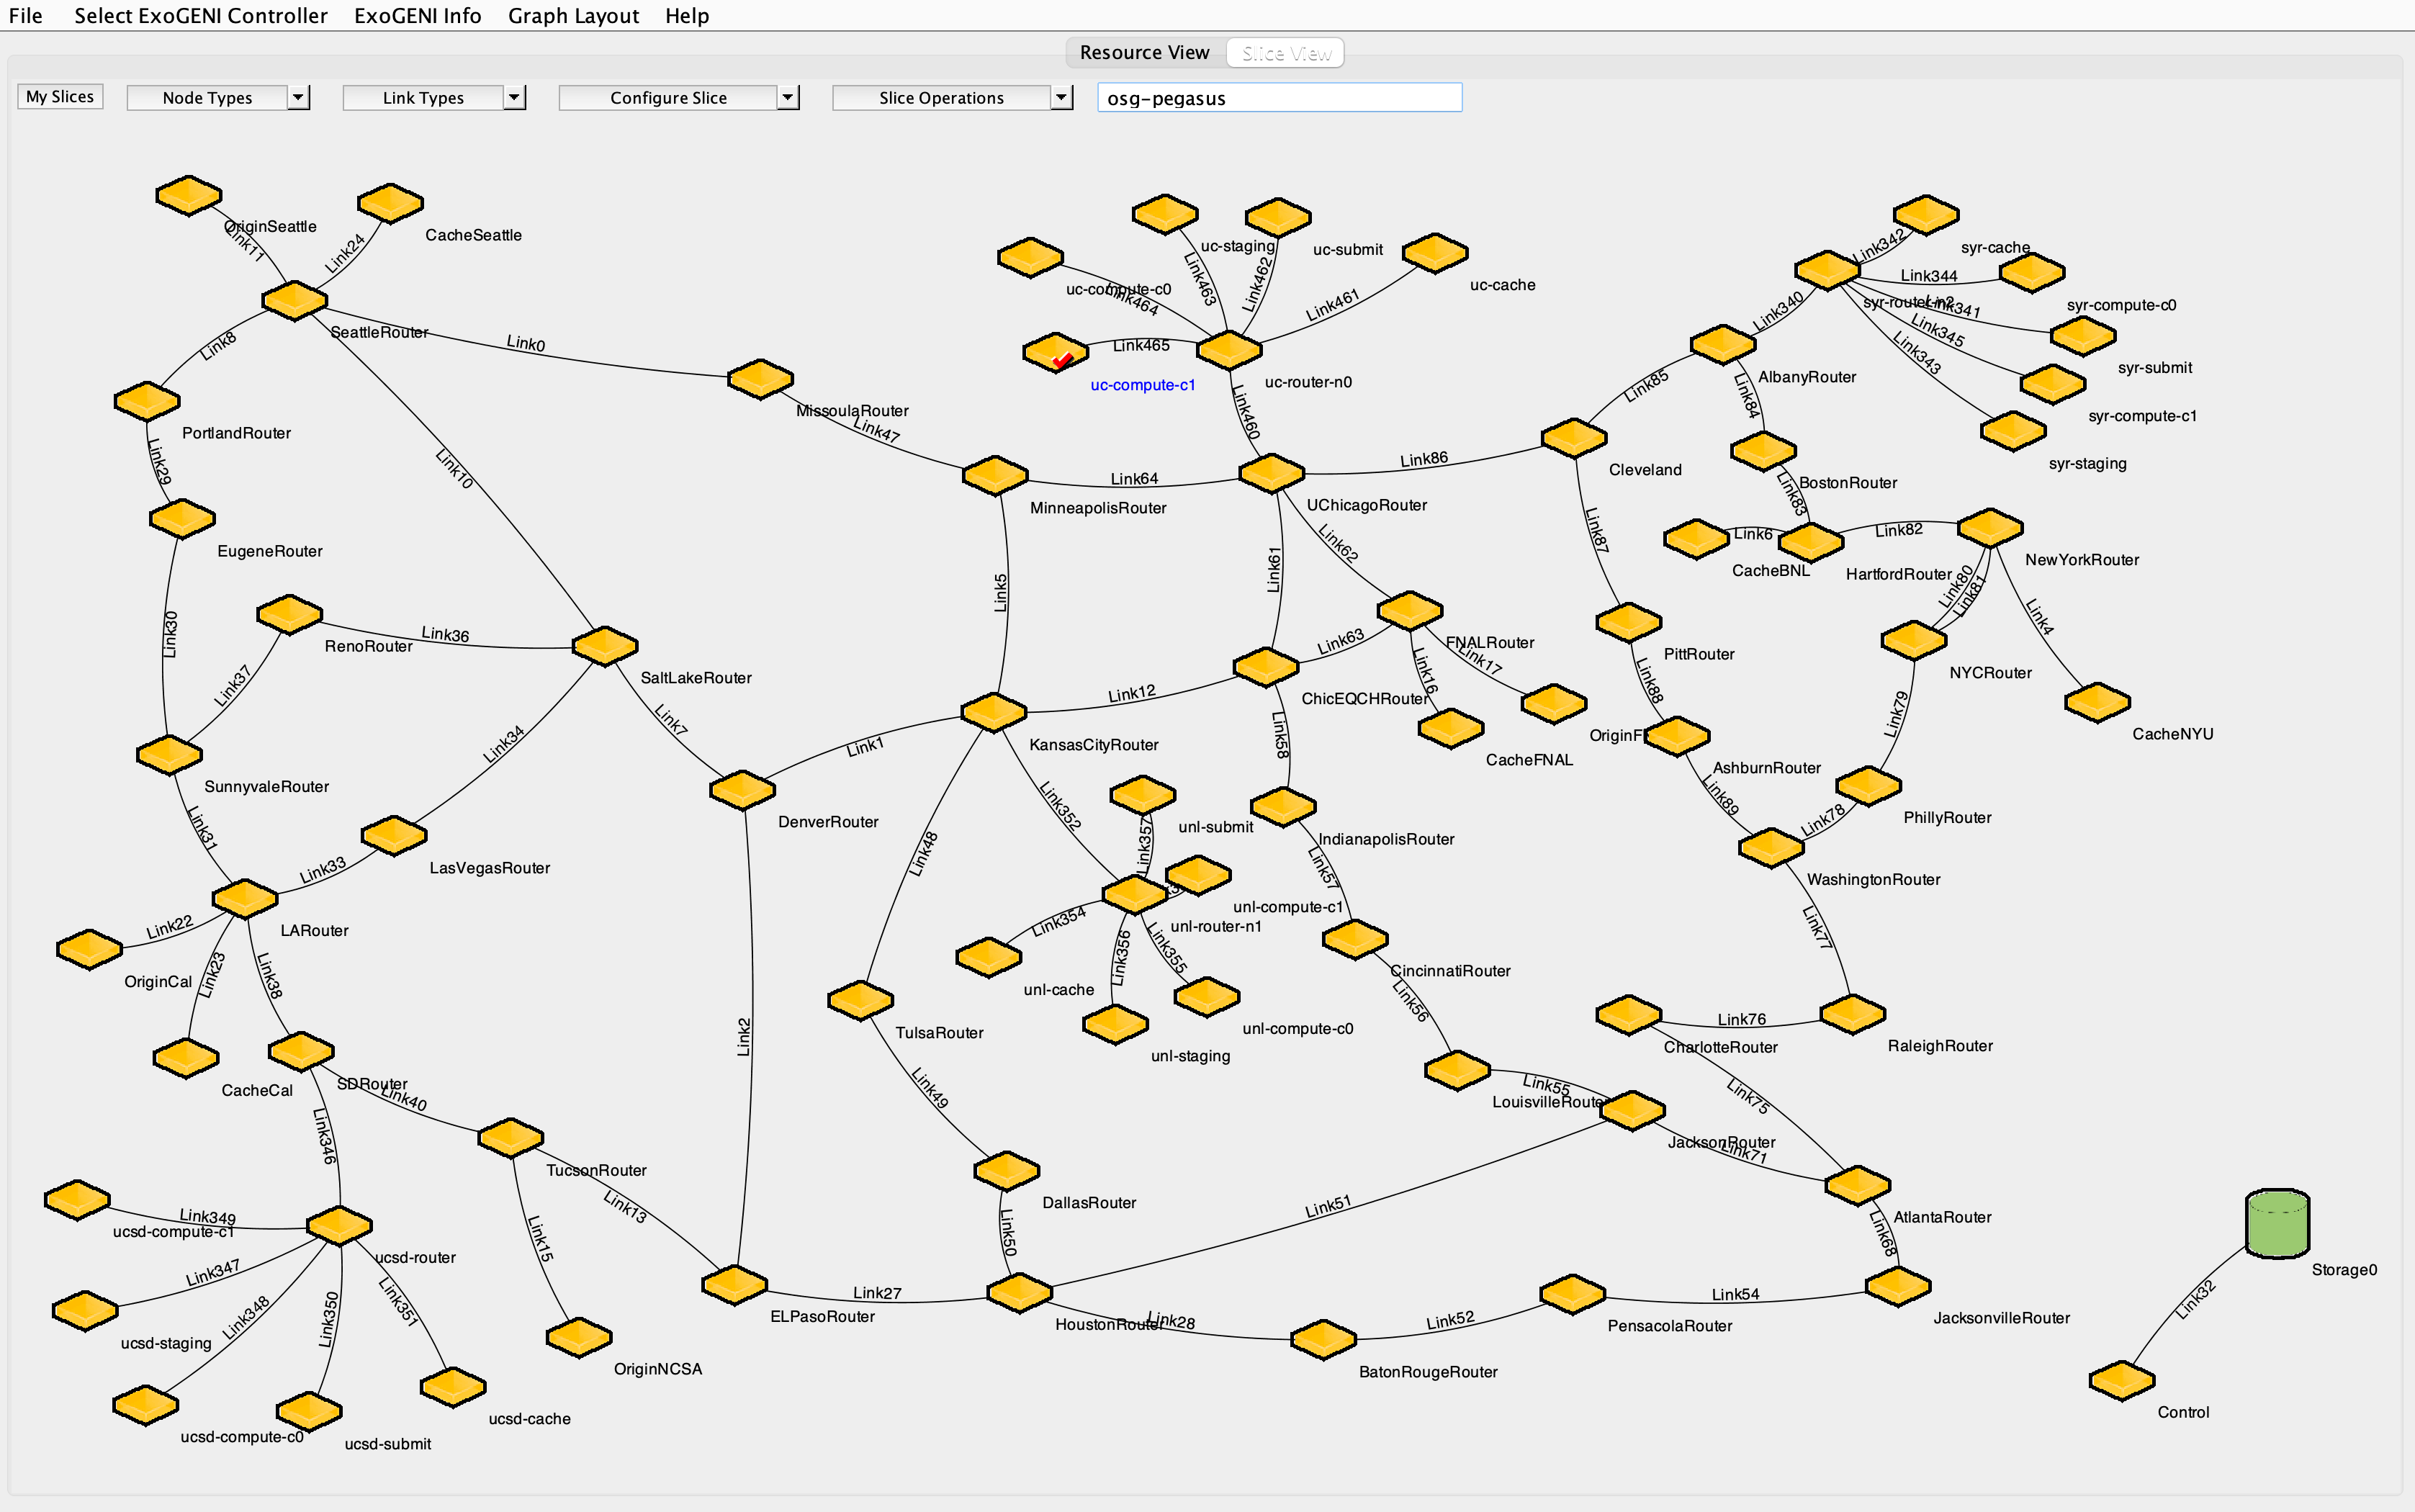
\includegraphics[width=0.4\textwidth]{./figure/osg_pegasus_request.png}
\end{center}
\caption{Emulation Network Topology}
\label{fig:topology}
%\vspace{-0.1in}
\end{figure}

To emulate the missing data, for a given missing rate, the mark vector $M$ is generated randomly and applied to the data site to create the 
missing data in the input matrix. The imputation performance is measured by the root mean square error (RMSE) between the original training data and the data recovered by the imputation algorithm. 

%If there are $n$ samples in the data set,
%\begin{flalign}\label{eq:rmse}
%\begin{aligned}
%RMSE = \sqrt{\frac{1}{n} \sum_{i=1}^{n}(\hat{X^i} - X^i)^2} \\
%\end{aligned}
%\end{flalign}

\subsection{Missing data imputation performance}
\label{subsec:im}
As we discussed in last section, the regression models with a regularization term are normally suitable to sparse input matrix.
We evaluated two representative $L_1$ regularization models, Ridge and Lasso with different penalty constant $\lambda$ in Fig.~\ref{fig:rmse:regu}.
When varying the missing rate from $5\%$ to $60\%$, $\lambda = 0.01$ for Ridge and $\lambda = 0.001$ and $\lambda = 0.0001$ for Lasso are the clear 
winners. Comparing the two figures, Lasso performs better than the Ridge counterpart.

  \begin{figure}[!ht]
    \subfloat[Imputation with Ridge\label{rmse:ridge}]{%
      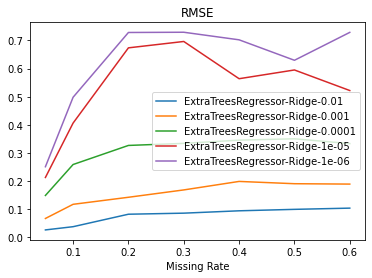
\includegraphics[width=0.23\textwidth]{./figure/rmse_ridge_1.png}
    }
    \hfill
    \subfloat[Imputation with Lasso\label{rmse:lasso}]{%
      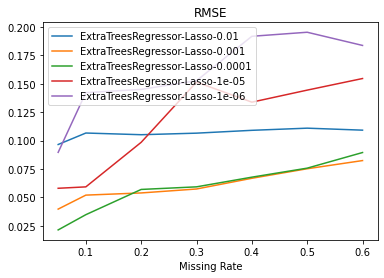
\includegraphics[width=0.23\textwidth]{./figure/rmse_lasso_1.png}
    }
    \caption{Imputation with Regularized Regressors}
    \label{fig:rmse:regu}
  \end{figure}

We further evaluate three other regressors against the tuned Lasso and Ridge regressors in Fig.~\ref{rmse:im}. It confirms that the Lasso with small 
penalty constant ($\lambda = 0.0001$) outperform all other regressors except for the cases of very low missing rate. The BayesianRidge regressor performs 
closest to Lasso, the K-Neighbors regress the second, and the ExtraTrees regressor the next. When the missing rate is low ($<20\%$), the ExtraTrees regressor 
performs much better than the other algorithms.

  \begin{figure}[!ht]
    \subfloat[Different Imputation Algorithms\label{rmse:im}]{%
      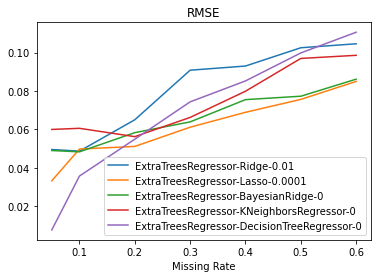
\includegraphics[width=0.23\textwidth]{./figure/rmse1.png}
    }
    \hfill
    \subfloat[Different Prediction Algorithms with Lasso Imputation\label{rmse:br}]{%
      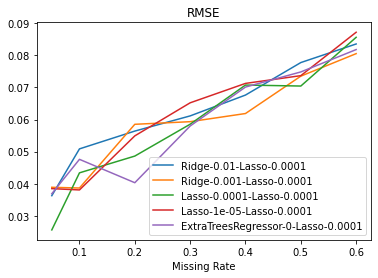
\includegraphics[width=0.23\textwidth]{./figure/rmsebr1.png}
    }
    \caption{Imputation Performance}
    \label{fig:rmse}
  \end{figure}

Since we implement the imputation regressor in the pipeline consisting of the ultimate prediction model, we also tried different prediction algorithms 
with the best Lasso imputation regressor. From Fig.~\ref{rmse:br}, their impacts on the imputation performance seem to be small, though different 
with different missing rates.
 
As we discussed in last section, the latest GAN based imputation algorithms showed some promising results in the medical domain. 
We applied the Generative Adversarial Imputation Nets (GAIN) developed in~\cite{Yoon2018GAINMD} to our data set and compared its performance 
with Lasso in Table~\ref{tab:gain}. The results actually do not the GAIN model outperforms the Lasso algorithm. We'll leave the further validation and 
customization of GAN framework to our future work.
  
 \begin{table}[!ht]
\caption{RMSE vs. Missing Rate) }
\label{tab:gain}
%\vspace{-0.1in}
\begin{center}
\begin{tabular}{ |c|c|c|c|c|c|c| } 
 \hline
  & 0.1 & 0.2 & 0.3 & 0.4 & 0.5 & 0.6\\ 
 \hline
  \hline
 GAIN & 0.1872 & 0.1794 & 0.214 & 0.2194 & 0.2666 & 0.2986 \\ 
 \hline
 Lasso & 0.05 & 0.0512 & 0.0612 & 0.0689 &0.0756 & 0.085\\
 \hline
\end{tabular}
\end{center}
%\vspace{-0.1in}
\end{table} 

\subsection{Inference performance with imputed missing data}
Many missing data imputation studies stoped after evaluating imputation performance as we did in subsection~\ref{subsec:im}. 
However, our ultimate goal is to improve inference accuracy of failure localization. In Fig.~\ref{fig:score}, we first evaluate the 
regression performance with different prediction algorithms on the best Lasso imputation regressor in terms of the 
coefficient of determination $R^2$ (Score) and the mean squared error (MSE) on the predicted output, the component 
failure probability vector $Y$ in Eq.~(\ref{eq:inverse}). We recall the higher score (best 1) and lower MSE mean better regression performance. 

  \begin{figure}[!ht]
    \subfloat[Prediction Score\label{score:t}]{%
      \includegraphics[width=0.23\textwidth]{./figure/score_test_train_1.png}
    }
    \hfill
    \subfloat[Prediction MSE\label{mse:t}]{%
      \includegraphics[width=0.23\textwidth]{./figure/mse_test_train_1.png}
    }
    \caption{Prediction Performance with Missing Data Imputation}
    \label{fig:score}
  \end{figure}
  
  The two metrics show the ExtraTrees regressor actually achieves the highest score and lowest MSE. The Ridge regressor with 
  small penalty constant ($0.01$) results the worst performance. The Ridge with
  bigger penalty constant ($0.1$) the the Lasso with very small penalty constant ($0.000001$) result in similar performance, 
  not far from the ExtraTrees algorithm. 
  
  We proceed to attempt to determine the failure locations with above combinations of prediction and imputation algorithms.
  For each test sample, after the predicted component failure probability vector $\hat{Y}$ is calculated, we sort the vector 
  elements in the descending order. In anticipating higher missing rate will likely significantly deteriorate the localization accuracy, 
  we evaluate the $Top-K$ accuracy with small number $k\le4$, which counts the correct label falls in the first $k$ elements in the 
  sorted $Y$ vector. Fig.~(\ref{fig:topk}) shows the localization accuracy when $k=1,2,3,4$. 
  
  The results are promising. For the exact match ($Top-1$) in Fig.~(\ref{a:t:1}), two best algorithms achieves over 
  $50\%$ accuracy at the missing rate $60\%$. When the missing rate is higher than $40\%$, the Ridge (0.1)+Lasso combination starts to outperform the ExtraTrees+Lasso algorithm, whose performance drops below the Ridge (0.01)+Lasso algorithm when $k>1$. The results show some disparities from the regression performance results in Fig.~\ref{fig:score}. 
   
    \begin{figure}[!ht]
    \subfloat[Top-1 Accuracy\label{a:t:1}]{%
      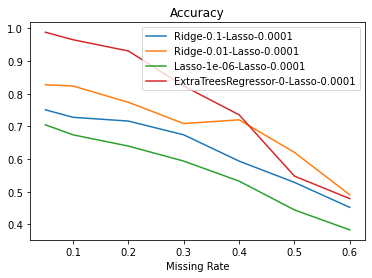
\includegraphics[width=0.23\textwidth]{./figure/Accuracy_test_train_1.png}
    }
    \hfill
     \subfloat[Top-2 Accuracy\label{a:t:2}]{%
      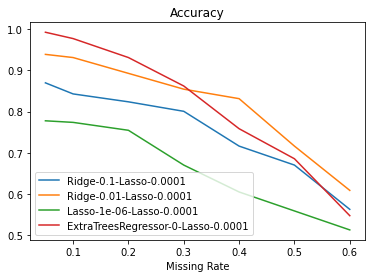
\includegraphics[width=0.23\textwidth]{./figure/Accuracy_test_train_2.png}
    }
    \hfill
      \subfloat[Top-3 Accuracy\label{a:t:3}]{%
      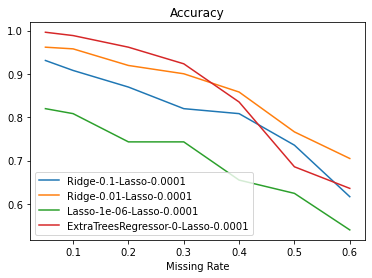
\includegraphics[width=0.23\textwidth]{./figure/Accuracy_test_train_3.png}
    }
    \hfill
   \subfloat[Top-4 Accuracy\label{a:t:4}]{%
      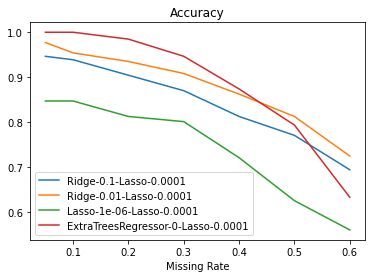
\includegraphics[width=0.23\textwidth]{./figure/Accuracy_test_train_4.png}
    }
    
    \caption{Top-k Classification Accuracy With Imputed Missing Data}
    \label{fig:topk}
  \end{figure}
  
  %\subsection{Prediction performance with missing whole features}
  
  %\begin{figure}[!ht]
  %  \subfloat[Prediction MSE\label{mse:nc}]{%
  %    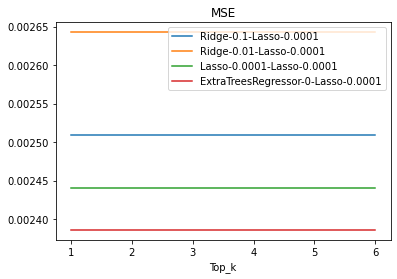
\includegraphics[width=0.23\textwidth]{./figure/MSE_test_nc_2.png}
  %  }
  %  \hfill
  %  \subfloat[Prediction Accuracy\label{accuracy:nc}]{%
  %    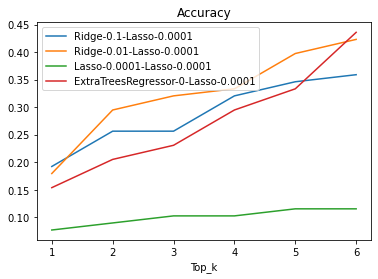
\includegraphics[width=0.23\textwidth]{./figure/Accuracy_test_nc_2.png}
  %  }
  %  \caption{Prediction Performance with Missing Whole Features}
  %  \label{fig:mse:regu}
  %\end{figure}
  